\documentclass[french]{rtxreport}

\usepackage{listings}
\usepackage[utf8]{inputenc}

\author{David Pineau}
\title{Documentation Technique}

\rtxdoctype{Documentation Technique}
\rtxdocref{technical\_documentation}
\rtxdocversion{0.1}
\rtxdocstatus{Release}

\rtxdochistory{
0.1 & 16/04/2011 & David Pineau & Traduction de la version anglaise \\
0.2 & 18/08/2011 & David Pineau & Traduction de la description
                                  d'implementation du cache         \\
}

\newcommand{\note}[1]{\marginpar{\scriptsize{\textdagger\ #1}}}



\definecolor{lstbackground}{rgb}{0.95, 0.95, 0.95}
\definecolor{lstcomment}{rgb}{0, 0.12, 0.76}
\definecolor{lstkeyword}{rgb}{0.66, 0.13, 0.78}
\definecolor{lststring}{rgb}{0.67, 0.7, 0.13}
\definecolor{lstidentifier}{rgb}{0.1, 0.1, 0.1}

\lstset{
        tabsize=2,
        captionpos=b,
        emptylines=1,
        frame=single,
        breaklines=true,
        extendedchars=true,
        showstringspaces=false,
        showspaces=false,
        showtabs=false,
        basicstyle=\color{black}\small\ttfamily,
        numberstyle=\scriptsize\ttfamily,
        keywordstyle=\color{lstkeyword},
        commentstyle=\color{lstcomment},
        identifierstyle=\color{lstidentifier},
        stringstyle=\color{lststring},
        backgroundcolor=\color{lstbackground}
}

\definecolor{grey}{rgb}{0.90,0.90,0.90}
\definecolor{rBlue}{rgb}{0.0,0.24,0.96}
\definecolor{rRed}{rgb}{0.6,0.0,0.0}
\definecolor{rGreen}{rgb}{0.0,0.4,0.0}

\lstdefinelanguage{rtx}%
{
	morekeywords={DECLARE, SEQUENCE, INTERFACE, IMPLEMENTATION, FROM, READ,
        OPTIONAL, CONFIGURATION_VARIABLE, USE, AS, WITH, SEQUENCES, ON, ELSE,
        LET, PROVIDES, REQUIRE, THROWS, FINALLY, FOREACH, IN, AND, OR, THROW,
        HANDLE_ERROR, NOT, REGISTER, LIKE, BIT, INTEGER, DOUBLE, BOOLEAN,
        STRING, MAPPED_AT, PCI},%
	sensitive=true,%
	morecomment=[l][\color{rRed}]{//},%
 	morecomment=[l][\color{rRed}]{\#},%
	morecomment=[s][\color{rRed}]{/*}{*/},%
	morestring=[b][\color{rGreen}]",%
	morestring=[b][\color{rGreen}]',%
	keywordstyle={\color{rBlue}}%
}[keywords,comments,strings]

\lstdefinelanguage{rti}%
{
	morekeywords={interface,
        builtin,
        type, sequence, variable,
        provided, required, optional},%
	sensitive=true,%
	morecomment=[l][\color{rRed}]{//},%
 	morecomment=[l][\color{rRed}]{\#},%
	morecomment=[s][\color{rRed}]{/*}{*/},%
	morestring=[b][\color{rGreen}]",%
	morestring=[b][\color{rGreen}]',%
	keywordstyle={\color{rBlue}}%
}[keywords,comments,strings]

\lstdefinelanguage{blt}%
{
	morekeywords={template,
        decl, stmt},%
	sensitive=true,%
	morecomment=[l][\color{rRed}]{//},%
 	morecomment=[l][\color{rRed}]{\#},%
	morecomment=[s][\color{rRed}]{/*}{*/},%
	morestring=[b][\color{rGreen}]",%
	morestring=[b][\color{rGreen}]',%
	keywordstyle={\color{rBlue}}%
}[keywords,comments,strings]





\begin{document}

\maketitle

\rtxmaketitleblock

\tableofcontents

\begin{abstract}
    Ce document décrit le fonctionnement du compilateur \rtx, en commençant par
    les différentes étapes du processus de compilation, jusqu'aux détails
    d'implémentation.  \end{abstract}


%\section*{Introduction}
%% What is Rathaxes
%% What is this document about exactly



\chapter{Les outils de \rtx}

\section{Le langage : CodeWorker}

\emph{CodeWorker} est un outil d'analyse et de génération de code, disponible
en logiciel libre (distribué sous GNU Lesser General Public License), et
développé par Cédric Lemaire. Il est destiné à couvrir plusieurs aspects de la
programmation générative. La programmation générative est une approche de
l'ingénierie logicielle qui a pour but de produire des systèmes informatiques
réutilisables, taillés sur mesure, faciles à faire évoluer et robustes, le tout
avec un haut niveau d'automatisation. Plus simplement, \emph{CodeWorker} est un
outil qui permet de générer du code en analysant des langages existants, ou en
permettant de créer son propre langage. Nous l'utilisons dans ce seul but, en
tant que ''compilateur des compilateurs''. Une fois un fichier d'entrée
contenant la description d'un langage a été analysé, \emph{CodeWorker} propose
plusieurs techniques de génération de code.

Le langage de script de cet outil dirige le processus d'analyse et de génération
de code source. Sa syntaxe est dérivé de la famille des langages proches du C,
en faisant un langage familier et facile à aborder pour la plupart des
programmeurs. La syntaxe de modèle de code (ou template) est proche des langages
JSP, ASP ou Velocity. Il possède des variations pour l'analyse, la génération,
et la programmation procédurale, offrant au développeur un grand nombre de
possibilités pour organiser des projets Codeworker.

\emph{CodeWorker} est plus puissant et plus facile à utiliser que
\emph{Lex/Yacc}, et correspond parfaitement aux besoins de génération de code
de \rtx. Il permet notamment de surcharger des règles d'analyse et de
génération de code existante, ce que peu d'outils similaire proposent. Ce
langage de scripting peut donc être divisé en trois majeures parties :

\begin{itemize}
    \item Language de description de \emph{BNF} : le langage d'analyse
        syntaxique de \emph{Codeworker} requiert une simple description BNF du
        langage à analyser, et chaque règle BNF est surchargeable dans un
        objectif d'extension du langage. Le DSL de rathaxes sera ainsi décrit ;
    \item Langage de script : les scripts \emph{Codeworker} sont suffisamment
        puissants pour les besoins de décoration d'AST de \rtx ;
    \item Langage de script de génération : Nous l'utiliserons pour les
        fonctionnalités de générations de code C de \rtx.
\end{itemize}



\section{La bibliothèque CNorm}

\emph{CNorm} est une bibliothèque d'analyse de C écrite en \emph{CodeWorker} par
Lionel Auroux (Directeur du Laboratoire Système et sécurité Epita/Epitech).
Cédric Lemaire (Auteur et développeur de \emph{CodeWorker}), David Giron, David
Amsallem et Christophe Fajardo (tous les trois de l'équipe de \rtx 2009). Elle
contient aussi toute une batterie de fonctions de script permettant de manipuler
un AST de C normalisé, afin de pouvoir générer le code C correspondant.

Cet outil a été pensé pour être aussi puissant que possible, afin de pouvoir
gérer n'importe quel dialecte du C (des extensions avec des qualifieurs et
spécifieurs spécifiques).

On y retrouvera donc les dialectes suivants :
\begin{itemize}
    \item Standard C 89 ;
    \item expressions assembleur GnuC ;
    \item Spécifieur \texttt{\_\_thread} pour catégorie de stockage GnuC ;
    \item Déclaration avancée de paramètre GnuC ;
    \item Qualifieur GnuC \texttt{\_\_extension\_\_} évitant des warnings pour
            les extensions GnuC ;
    \item Sous-script GnuC ;
    \item Initialiseurs désignés GnuC ;
    \item Builtin GnuC \texttt{\_\_builtin\_offsetof} ;
    \item Builtin GnuC \texttt{\_\_builtin\_va\_list} ;
    \item c99 : mot clef \texttt{static} dans la règle de déclarateur
                absolu direct ;
    \item Bloc de code c99 en tant qu'expression (\texttt{\{ \}}) ;
    \item c99 : \texttt{typeof} ;
    \item c99 designation ;
    \item c99 : \texttt{\_\_alignof} ;
    \item c99 : \texttt{complex}, \texttt{\_\_real} ;
                \& \texttt{\_\_imag operator} ;
    \item c99 : expression de portée ; %range expressions
    \item c99 et attributs Windows ;
    \item Syntaxe K. \& R. du C ;
    \item Types manquants dans les déclarations de fonctions.
\end{itemize}

Cette grammaire a été adaptée à partir de celle trouvable dans la section A13
du livre ''C Programming Language'', seconde édition, par Brian W. Kenighan et
Dennis M. Ritchie (Englewood Cliffs, New Jersey: Prentice Hall PTR, 1988; ISBN
0-13-110362-8), pages 234 - 238. 

Cnorm est utilisé dans \rtx afin d'analyser le code C présent dans la partie
backend du DSL, afin d'éviter des données opaques, et d'offrir un contrôle
précis sur le code manipulé. Elle est aussi utilisée pour la génération finale
de code C des pilotes. La structure de l'arbre de syntaxe abstraite C (AST) peut
être trouvée dans la documentation du Cnorm, et nous ne l'aborderons pas ici.


\chapter{Cas d'utilisation de \rtx}

\section{Les utilisateurs}

Comme décrit dans l'introduction, \rtx vise principalement deux types de
développeurs.

La cible principale est le développeur de pilote de périphérique. C'est lui qui
écrira le code décrivant les algorithmes à implémenter pour le périphérique pour
lequel il veut générer le code.

La seconde cible est le développeur noyau. Son rôle est d'implémenter et de
fournir la bibliothèque de modèles de codes C qui contiennent le code
spécifique à chaque système d'exploitation.

Finalement, un troisième type de développeur apparait avec un autre rôle précis
dans le processus de génération d'un pilote de périphérique en C. En utilisant
la documentation sur l'état de l'art du développement de pilotes, il définira
des interfaces que tous les systèmes d'exploitation respectent en dégageant la
sémantique de chaque concept intervenant dans le développement d'un pilote. Ces
interfaces devront êtres respectées par les deux autres types de développeurs,
afin d'assurer la cohérence du code et donc du pilote généré.

\section{Un DSL en trois parties}

Comment on peut donc le voir, trois types de développeurs vont interagir avec
\rtx, et le faire évoluer, chacun pouvant se focaliser sur une partie spécifique
du langage dédié. Chacun de ces trois parties a sa propre place et sa fonction
au sein du processus de génération du code C d'un pilote de périphérique.

\subsection{Mainteneur \rtx : Middle-End}
\lstset{language=rti}

Tout d'abord, bien que cela ne soit pas le type de contributeur au langage le
plus visible, le mainteneur \rtx n'en est pas moins l'un des plus importants.
En effet, comme expliqué au préalable, son rôle est de définir des interfaces
qui devront être respectées dans les deux autres parties du langage \rtx.

Ces interfaces font partie ce que que nous appelons le \emph{Middle-End} du
langage. Il pourrait être vu comme une description interne du compilateur de ce
qui est requis ou optionnel au sein de la description algorithmique du
périphérique, ainsi qu'au sein des modèles de code spécifiques aux systèmes.
C'est ce qui va servir de lien entre les deux autres parties : le Front-end et
le Back-end, en définissant tous les types, séquences ou variables disponibles.

L'extension d'un fichier contenant des interfaces est \texttt{.rti} pour \rtx
Interface.

Une interface est identifiée par un nom unique au sein du compilateur, qui
généralement correspond au type de sous-système qu'elle décrit.

Elle contient donc :
\begin{itemize}
    \item Les types utilisés dans le sous-système, qui doivent être fournis par
        les modèles de code C ;
    \item Les séquences (fonctions ou algorithmes) qui sont fournies par les
        modèles de code C ;
    \item Les séquences (fonctions ou algorithmes) qui sont requis ou optionnels
        et doivent être fournis par la description algorithmique du
        périphérique ;
    \item Les variables ou valeurs de configuration requises par l'interface.
\end{itemize}

Par exemple, nous pourrions avoir :
\begin{itemize}
    \item Interface Userland : décrit les fonctions et types faisant partie
        d'un module noyau chargeable ;
    \item Interface PCI : décrit les fonctions et types du BUS PCI ;
    \item Interface IO : décrit les fonctions qui peuvent être utilisées pour
        un pilote de périphérique branché en port IO.
\end{itemize}

Voici un exemple de ce à quoi ressemble une interface :
\begin{lstlisting}
    interface Userland
    {
        // Here a list of compiler-builtin types
        builtin type bit;
        builtin type byte;
        builtin type word;
        builtin type dword;
        builtin type qword;

        builtin type register;
        builtin type buffer;
        builtin type context;

        // Here a type that has to be implemented in the templates
        type device;

        // Here is a sequence provided by the templates
        provided sequence concat(register, buffer);

        // Here are the sequences asked from the .rtx file
        required sequence doSomething(context, register);
        optional sequence doNothing(device);

        // Here the variables required from the .rtx file
        required variable os;
        required variable version_major;
        optional variable version_minor;
    };
\end{lstlisting}

En réalité, cette partie du langage dédié est la seule partie qui se suffit à
elle même pour pouvoir être validée par le compilateur (hormis ses
dépendances). En effet, c'est la partie qui définit tous les types génériques
devant/pouvant être implémentés ou utilisés par le reste du langage.

\subsection{Développeur noyau : Back-End}
\lstset{language=blt}

En second vient un autre type de contributeur indispensable à \rtx : le
développeur noyau. C'est lui qui va implémenter les modèles de code C
spécifiques à chaque OS, pour chacune des interfaces existantes, permettant
ainsi de supporter une multitude de systèmes d'exploitation.

Le rôle du backend est donc de fournir le code spécifique au système
d'exploitation pour chaque interface existante, afin d'offrir le support du
système le plus complet possible. L'extension de ces fichiers est \texttt{.blt}
pour Backend Library Template .

En utilisant les interfaces présentes, le compilateur pourra indiquer ce qui est
supporté ou non pour un système d'exploitation particulier, ainsi que faire de
la vérification de typage, indiquant si l'utilisation des séquences et des types
est lexicalement correcte ou non.

Le code template est contenu dans un bloc \emph{with} qui associe le code
spécifique qu'il contient à des variables de configuration avec des valeurs
spécifiques. Cela signifie que que ce code spécifique ne sera utilisé que
lorsque les variables de configuration respectent les conditions écrites.

À l'intérieur du bloc \emph{with} peuvent se trouver un ou plusieurs modèles de
code C. Un modèle (ou template) est identifié par son type. C'est ce qui permet
le référencement de templates entre eux.

Le contenu d'un template est en réalité du C instrumenté selon les besoins de
rathaxes. Ce code C peut être ou non spécifique à la plate-forme et à un système
d'exploitation. Instrumenté signifie bien entendu que le C a été étendu pour
permettre les fonctionnalités de génération de rathaxes, où des variables
peuvent influencer la génération de code. Cette surcharge de la syntaxe du C
permet aussi bien la concaténation de code (ou d'identifiants) que des appels
entre templates.

Voici un petit exemple de ce à quoi cela peut ressembler :
\begin{lstlisting}
    with os=Linux, version >= 2.6, bus=ioport
    {
        template get(register reg) decl
        {
            ${register} get_reg_${reg.name}(void)
            {
                return in${reg.basetype.initial}(${reg.addr});
            }
        }

        template get(register reg) stmt
        {
            get_reg_${reg.name}()
        }
    }
\end{lstlisting}

\subsection{Développeur de pilote : Front-End}
\lstset{language=rtx}

Finalement, le dernier mais aussi le plus évident des utilisateurs de \rtx est
le développeurs de pilotes de périphériques. Lui va interagir avec la partie du
langage dédié que nous appelons le frontend. C'est la section du langage qu'un
électronicien utilisera afin de décrire les algorithmes à utiliser pour le
pilote du périphérique. Cette partie du langage contient les syntaxes
nécessaires à la description de registres possédant des champs nommés (ou non),
ainsi que tous les utilitaires permettant de manipuler intelligemment ces
registres, sans oublier la possibilité d'écrire des algorithmes.

L'extension de fichier à utiliser pour cette partie du langage est
\texttt{.rtx} pour \rtx.

Un des aspects les plus importants du frontend est qu'il contient un bloc
appelé bloc de \emph{configuration}. C'est ce bloc qui détermine les valeurs
associées aux variables de configuration déclarées par les interfaces et
utilisées par le backend lors de la génération du code C du pilote.

Compiler un fichier \texttt{.rtx} signifie vérifier les types et la
disponibilité de chacun de ces types ainsi que des séquences en les comparant
aux interfaces du middleend. Se référer à la section
\ref{sec:driverCompilation} pour plus d'informations.



\chapter{Architecture du compilateur}

\section{Les composants}

Un compilateur n'est jamais un simple programme. Dans le cas de \rtx, nous
pouvons identifier différents éléments composant le cœur du compilateur.
Puisque la souplesse et l'évolutivité du langage est un de nos principaux
objectifs dans ce projet, ces composants étaient absolument nécessaires. Voici
un schéma les illustrant :

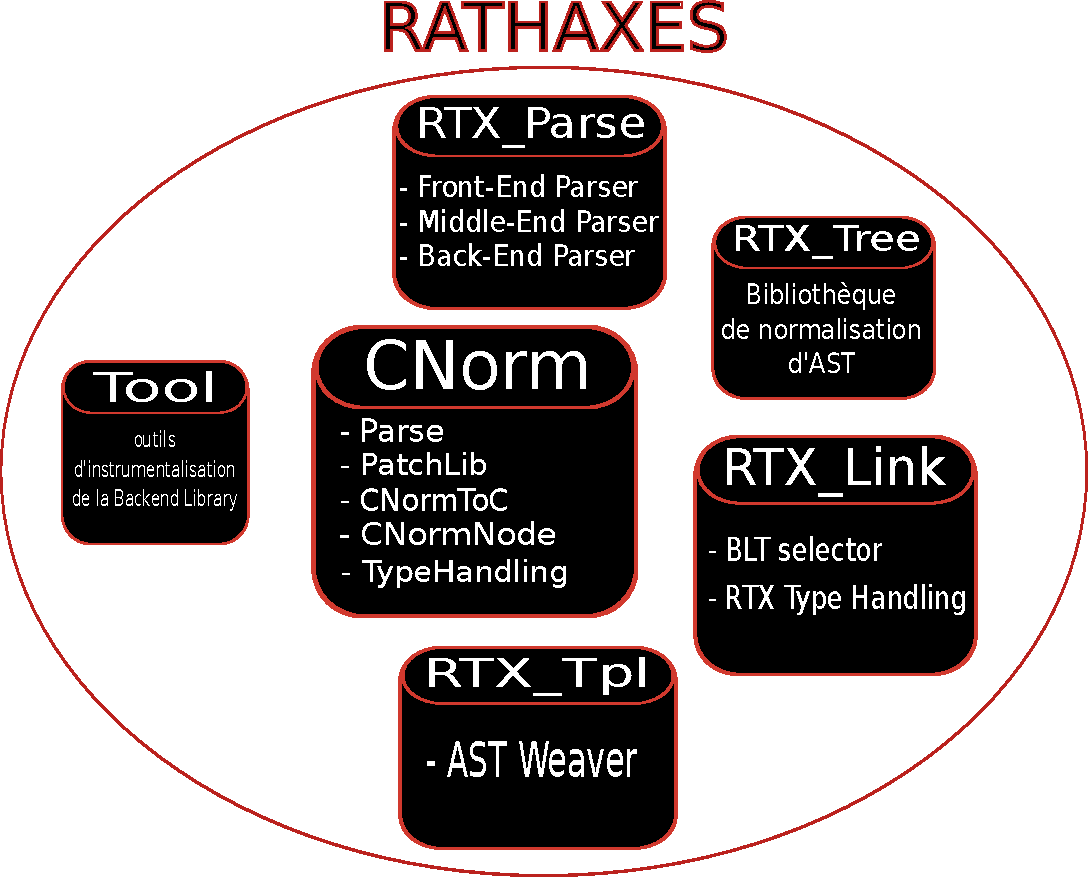
\includegraphics[width=0.95\textwidth]{diagramme_architecture.pdf}

Tout d'abord, la bibliothèque \emph{Cnorm} vue auparavant fait partie du
compilateur. Son rôle est tout d'abord de générer le code C final, mais c'est
aussi ce qui permet l'analyse du code C contenu dans les modèles de code du
backend, grâce aux fonctionnalités de surcharge de syntaxe de CodeWorker.

Le composant suivant, \emph{RTX\_Parse}, est le composant dont le rôle est
(comme son nom l'implique) l'analyse syntaxique de l'ensemble du langage. Il
construit ainsi un arbre de syntaxe abstraite.

\emph{RTX\_Tree} vient avec \emph{RTX\_Parse}, puisque c'est le composant qui
permet de normaliser l'AST généré. Ainsi, chaque type de nœud de l'arbre
respecte un format précis et fixé de représentation de données.

Ensuite, les deux composants \emph{RTX\_Link} et \emph{RTX\_Tpl} sont les
modules qui entrent en jeu lors du processus de transformation d'un AST \rtx en
AST C grâce a l'utilisation des modèles de code. Leur rôle sera détaillé plus
amplement dans la section \ref{sec:compilationSteps}.

Finalement, le module \emph{Tool} est un module plus utilitaire qu'autre chose.
En effet, il contient une série d'outils permettant de générer des fichiers
requis par les systèmes d'exploitation cibles, mais qui ne sont pas exactement
du code C. Par exemple, sur un système du type UNIX, il permettra de générer un
Makefile facilitant la compilation du code du pilote, tandis que sur un système
Windows, il permettra de générer un fichier \texttt{.inf} qui fournit des
information au noyau au sujet du module à charger.


\section{Les étapes de compilation}
\label{sec:compilationSteps}

De l'analyse syntaxique d'un fichier \texttt{.rtx} à la génération du code C
d'un pilote, l'AST va subir un certain nombre de transformations. Cependant,
les templates sont eux aussi compilés dans le but de les sauvegarder dans un
cache au sein du compilateur. Ceci mène à deux modèles de compilation : La
compilation d'un template, et la compilation d'un pilote.

\subsection{Template}

La compilation d'un template peut être divisée en plusieurs étapes, puisque la
compilation d'un template génère une représentation en AST ainsi que du code
CodeWorker. Ce code permettra de faire la résolution de toutes les variables
provenant du frontend lors de l'intégration de la représentation AST du
template au sein de l'AST du pilote.

On peut ainsi identifier les étapes suivantes :
\begin{enumerate}
    \item Analyse syntaxique : construction d'un AST normalisé par le Cnorm et
        RTX\_Tree;
    \item Identification des placeHolders : construction d'une node référençant
        chacun des placeHolder.
    \item Analyse des placeHolders : Construction d'une node pour chacun des
        placeHolders référencés.
    \item Génération de CodeWorker : génération de code CodeWorker dont le rôle
        est de résoudre les placeHolders a l'aide des variables templates
        provenant du frontend, permettant le tissage de l'AST du template dans
        l'AST du pilote final.
\end{enumerate}

Par la suite, le développeur pourra installer le template compilé au sein de la
bibliothèque backend du compilateur. Installer signifie qu'une entrée sera
ajoutée dans un cache au sein du compilateur, permettant de le retrouver lors
de la compilation d'un pilote.


\subsection{Pilote}
\label{sec:driverCompilation}

La compilation d'un pilote est un processus complexe, où chaque partie du DSL
est prise en compte.

Voici une liste des étapes de la compilation d'un pilote :
\begin{enumerate}
    \item Analyse syntaxique : construction d'un AST a partir du code frontend ;
    \item Vérification du typage : vérification des types utilisés dans le
        frontend par rapport aux types fournis par l'interface.
    \item Sélection de template : le composant RTX\_Link sélectionne dans le
        cache les templates correspondant aux variables de configuration
        provenant du frontend ; variables;
    \item Instanciation du template : le composant RTX\_Tpl instancie chaque
        template AST référencé par le frontend, et appelle la fonction
        CodeWorker de résolution des variables templates, avant de lier les
        deux AST ;
    \item Génération : génération du code C à partir de l'AST transformé ;
    \item Génération des outils : Le module \emph{Tool} génère les fichiers
        annexes nécessaires pour la bonne compilation des pilotes générés.
\end{enumerate}


\subsection{Processus de compilation général}

Comme vous avez pu le comprendre, si nous avons parlé de trois parties d'un
seul et même langage, c'est pour la simple et bonne raison que le compilateur
est capable de gérer les trois indifféremment. En effet, on pourrait dans
l'absolu écrire un pilote en partant de rien dans un seul et même fichier.
Cependant, cette possibilité est principalement réservée dans le but de faire
une suite de tests. De plus, les 3 principaux utilisateurs de \rtx se
concentreront normalement chacun sur une des trois parties du langage.

Ceci se ferait donc grâce à l'identification des mots clefs contenus dans le
fichier. Voici un schéma illustrant ce processus général :

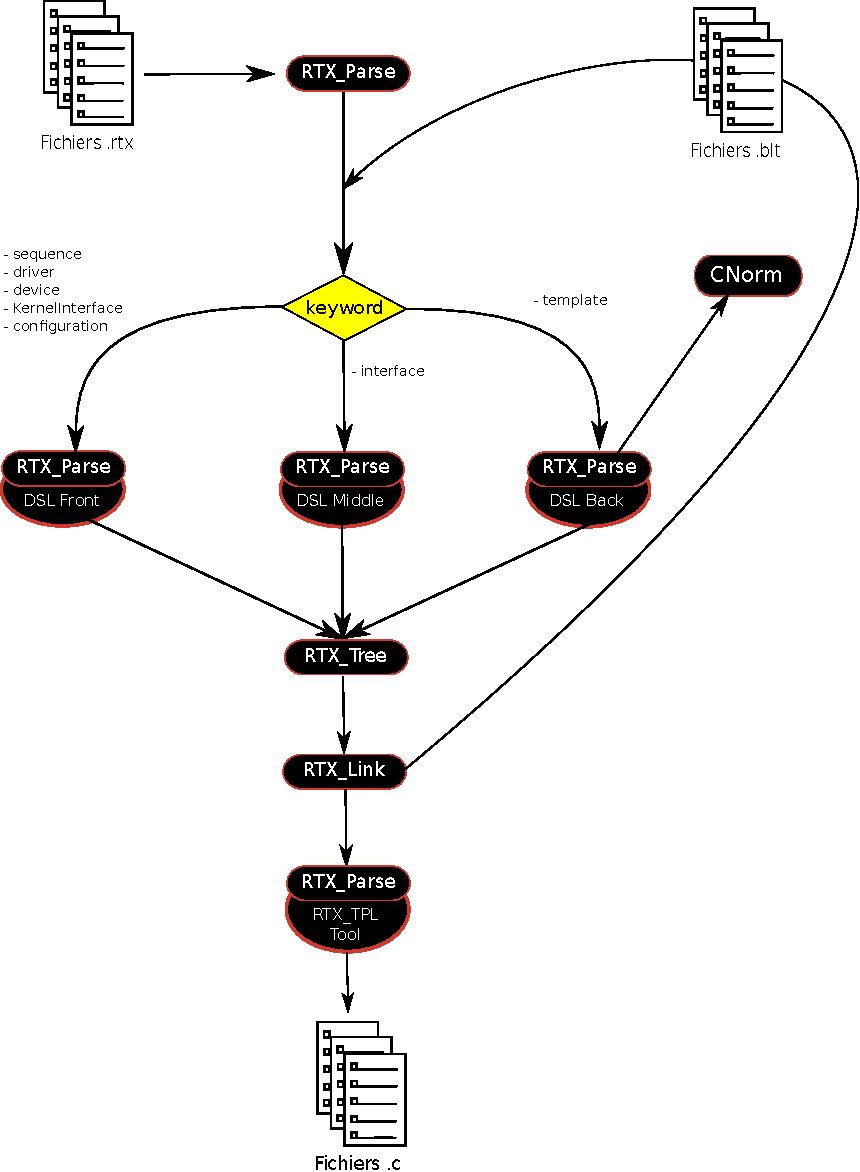
\includegraphics[width=0.95\textwidth]{logigramme.pdf}



\chapter{Details d'implementation}



\section{Cache de modeles pre-compiles}

Un des elements les plus importants du compilateur est le \emph{cache}. Au
travers de celui-ci, le compilateur peut maintenir une liste complete de
modeles de codes et d'interfaces pre-compilees, qui permettra de trouver
rapidement les templates a utiliser pour la compilation et la generation d'un
pilote.

CodeWorker utilise une variable globale appelee ``this'', ou l'on peut stocker
n'importe quelle information. Elle est en realite utilisee par rathaxes afin de
stocker le \emph{cache} et de le rendre accessible durant toute la phase de
compilation et de generation. Nous y stockons les informations suivantes :
\begin{enumerate}
    \item Les ``codes globaux'' enregistres
    \item Les templates enregistres
    \item Les chunks enregistres
    \item Un etat differentiel du cache
\end{enumerate}

Chacune de ces categories se traduit par un noeud contenu dans le champ
``session'' de la variable globale ``this'' de CodeWorker. Nous l'appelons la
session de cache.

Tout element enregistre est un bout de code pre-compile et verifie par le
compilateur avant son enregistrement. Ainsi, chacun d'entre eux est associe a
un fichier de script CodeWorker genere (qui a pour role la resolution de tous
les placeholders du code associe) ainsi qu'un fichier \texttt{.tree} contenant
l'AST correspondant. Ces deux elements peuvent etre optionnels pour certains
elements enregistres dans le cache.

Maintenant, nous allons decrire chacune de ces categories de maniere plus
detaillee, et expliquer leur role et leur utilisation.


\subsection{Codes globaux enregistres}

Les codes globaux enregistres sont contenus dans le champ ``.global\_code'' de
la session de cache.

Un ``code global'' est un bout de code specifique au sein de rathaxes : c'est
une sorte de \emph{chunk} hors d'un template, dont la selection est automatique
des le moment ou l'interface qui le contient est utilisee pour la generation
d'un pilote. c'est donc du code C instrumente contenu dans un bloc \emph{with}.

Seul un element de cette categorie peut etre charge pour une interface donnee.
Lors de la generation du pilote, chacun des codes globaux associes a chaque
interface sera automatiquement charge, resolu et tisse dans l'AST final, des le
moment ou leur interface est utilisee.

Lorsqu'un code global est enregistre dans le cache, il est insere en tant
qu'element dans une liste, ou chaque element contient les champs suivants :
\begin{itemize}
    \item ``.with'': Noeud decrivant les contraintes de configuration
        permettant la selection du morceau de code (C'est ausis l'element qui
        indique a quelle interface est associee le code global)
    \item ``.script\_file'': Champ obligatoire.
    \item ``.tree\_file'': Champ obligatoire.
\end{itemize}


\subsection{Template enregistres}

Les templates enregistres sont contenus dans le champ ``.templates'' de la
session de cache.

Ce champ est en realite un tableau associatif ou la clef est un hash du
prtottypedu template, et la valeur une liste des templates enregistres associes
a ce prototype. Cela permet de pouvoir conserver tous les templates, quelles
que soient leurs contraintes de selection, puis de faire le tri afin de
selectionner le bon template selon la configuration. Cela dit, deux templates
enregistres ne peuvent avoir de contraintes identiques : Celles-ci doivent
differer, et on permet ainsi d'eviter aussi bien des problematiques liees a la
selection du bon template, ainsi que des problematiques liees au
double-enregistrement d'un template.

Chaque template enregistre est un noeud contenant les champs suivants :
\begin{itemize}
    \item ``.with'': Noeud contenant les contraintes de selection du template
    \item ``.rtype'': Noeud contenant le prototype du template complet
    \item ``.chunks'': Liste d'objets decrivant les chunks contenus par le
        template.
    \item ``.script\_file'': Champ optionnel. Il n'est present que dans le cas
        ou le template est un template de type.
    \item ``.tree\_file'': Champ optionnel. Il n'est present que dans le cas
        ou le template est un template de type.
\end{itemize}

Chaque objet stocke dans le champ ``.chunks'' est un moyen d'indiquer ou est
stocke le \emph{chunk} dans le cache. Sa clef est le nom qualifie du pointcut
auquel il est associe, et la valeur est l'index correspondant au chunk contenu
par le template dans la list des chunks associes au pointcut donne. Plus
d'informations au sujet de la maniere de stocker les chunks sont donnees dans
la section suivante.


\subsection{Chunks enregistres}

Les chunks enregistres sont contenus par le champ ``.chunks'' de la session de
cache.

Ce champ est un tableau associatif, qui suit le meme modele que le tableau
associatif qu'est le champ ``.templates''. La clef est le nom du pointcut
qualifie (ex: ``interface::nom'' ou ``::nom'' s'il n'est associe a aucune
interface), et la valeur est une liste des chunks qui y sont associes. De la
meme maniere que pour les templates, les chunks contenus dans cette liste sont
uniques.

Chaque chunk enregistre contient lees champs suivants :
\begin{itemize}
    \item ``.with'': Noeud contenant les contraintes de selection du template
        contenant le chunk
    \item ``.name'': Nom qualifie du pointcut
    \item ``.tpl\_id'': Hash du template contenant le chunk
    \item ``.script\_file'': Champ obligatoire.
    \item ``.tree\_file'': Champ obligatoire.
\end{itemize}


\subsection{Etat Differentiel du cache}

Ce que nous appelons un ``etat differentiel du cache'' est en realite une sorte
de registre de toutes les modifications appliquees au cache durant le processus
de compilation. Ceci permet de pouvoir valider ou non l'enregistrement d'un
element au sein du cache, et de pouvoir retrouver quels sont els fichiers de
script et d'AST a sauvegarder ou non. C'est ce qui permet l'operation dite
"d'installation" d'un template ou d'une interface.

Le differentiel de cache est contenu dans le champ ``.temp'' de la session, et
a une structure similaire àa sessiond e cache elle meme, a cela pres que chacun
de ses elements enregistres est en realite  une reference sur l'element
enregistre dans la session de cache. C'est ce qui permet de les supprimer
facilement, et de les gerer comme n'importe quel element du cache durant un
processus de generation de pilote.

Lorsque le cache est valide, le compilateur, selon les argument qu'il a recus,
peut installer les fichiers nouvellement pre-compiles au sein du cache
persistant. Ce processus d'installation consiste en trois operations :
\begin{itemize}
    \item Calculer un nom de fichier a partir d'informations associes a
        l'element a enregistrer
    \item Copier les fichiers pre-compiles dans la bibliotheque de backend sous
        le nom calcule
    \item Mettre a jour les chemins de fichiers au sein du cache
\end{itemize}

Grace au differentiel de session, ces operations sont facilement effectuees, et
le cache peut rester coherent.


\subsection{API de manipulation du cache}

Dans cette section sont decrites toutes les fonctions ``publiques'' du cache,
de maniere a permettre la maintenant de son code et son utilisation plus aisee.
Chacune de ces fonctions se trouve dans le fichier rtxLink.inc.cws des scripts
du compilateur.

Tout abord, il est necessaire de comprendre que le cache a deux possibles cas
d'utilisation : le remplir avec des fichiers que l'on vient de pre-compiler, ou
en tirer des informations necessaires a la generation d'un pilote.

\vspace{20pt}

Les fonctions a utiliser pour les deux cas d'utilisation sont les suivantes :

\begin{lstlisting}
function rtxLink_LoadCache();
\end{lstlisting}
La fonction \emph{rtxLink\_LoadCache} est utilisee pour charger le cache en
memoire depuis un fichier contenant sa description, qui se trouve dans la
bibliotheque de backend. Si cette fonction n'est pas appelee avant un autre
appel au cache, il sera considere comme vide, et effacera l'ancien cache si il
devait par hasard etre sauvegarde.

\begin{lstlisting}
function rtxLink_SaveCache();
\end{lstlisting}
La fonction \emph{rtxLink\_SaveCache} est utilisee pour sauvegarder le cache
dans un fichier situe dans la bibliotheque de backend, afin de le rendre
persistant. Si une quelconque modification a ete apportee au cache avant un
appel a cette fonction, elle se chargera automatiquement de sauvegarder les
fichiers temporaires correctement au sein de la bibliotheque du backend et de
mettre a jour le cache persistant.

\begin{lstlisting}
function hashTemplatePrototype(theRType     : node,
                               out_ref_hash : reference);
\end{lstlisting}
La fonction \emph{hashTemplatePrototype} prend en premier argument une node
decrivant le prorotype du template et en second argument une reference
permettant de renvoyer le hash du prototype. Cette fonction est utilisee de
maniere eparse dans le code, afin de maintenir une coherence dans le hash
utilise pour les templates.

\vspace{20pt}

Les fonctions suivantes sont utilisees afin d'inserer des elements dans le
cache.

\begin{lstlisting}
function rtxLink_RegisterToCache(local_node : node);
\end{lstlisting}
La fonction \emph{rtxLink\_RegisterToCache} traverse un AST rathaxes dans son
ensemble, et enregistre chaque bloc au sein du cache (code global, template,
chunks).

\vspace{20pt}

Les fonctions suivantes sont utilisees pour manipuler le cache, afin de
resoudre des placeholders et de generer du code. Nous pouvons alors identifier
quatre cas d'utilisation : Resolution d'un \emph{pointcut} (instanciation de
tous les chunks selectionnes associes), resolution d'un code global, resolution
d'un chunk au travers du template associe (mecanisme interne tels que l'appel
d'une sequence), et finallement la resolution d'un mapping de template de type.

\begin{lstlisting}
function rtxLink_findGlobalCode(with_values  : node,
                                out_code_ref : reference);
\end{lstlisting}
La fonction \emph{rtxLink\_findGlobalCode} recupere le noeud d'un code global
correspondang a la configuration ``with\_values'' et la retourne grace a la
reference donnees en second parametre.

\vspace{20pt}

fonctions utilisees pour resoudre un template (ou un de ses chunks) :
\begin{lstlisting}
function rtxLink_findTemplates(theRtype : node,
                               out_tpls : node);
\end{lstlisting}
La fonction \emph{rtxLink\_findTemplates} recupere la liste complete des
templates associes a un prototype decrit par le parametre ``theRtype'' et la
copie dans le parametre ``out\_tpls''.

\begin{lstlisting}
function rtxLink_selectUniqueTemplate(templates : reference,
                                      config : node);
\end{lstlisting}
La fonction \emph{rtxLink\_selecteUniqueTemplate} selectionne un template
unique dans la liste de templates donnes dans le parametre ``templates'',
recuperee au travers de la fonction \emph{rtxLink\_findTemplates} en fonction
de la configuration contenue par le parametre ``config''. Le template
selectionne est alors reference dans le parametre ``templates'' pour le retour.
En cas d'echec, la fonction renvoie ``false''.

Dans le cas d'une resolution de mapping de template de type, la node ainsi
recuperee peut etre directement envoyee a la fonction
\emph{rtxLink\_LoadScript}, qui chargera l'arbre et le script associes.

\begin{lstlisting}
function rtxLink_selectChunkFromTemplate(theTemplate : node,
                                         chunkName : value,
                                         theChunk : reference);
\end{lstlisting}
La fonction \emph{rtxLink\_selectChunkFromTemplate} prend une node de template
recuperee grace a la fonction \emph{rtxLink\_SelectUniqueTemplate} ainsi qu'un
nom qualifie de \emph{pointcut} par le parametre ``chunkName''. Elle va alors
aller chercher le chunk associe au template portant le nom demande. Si aucun
chunk associe ne porte ce nom, elle renvoie ``false''. S'il existe un chunk
associe mais qu'il n'est pas trouve, alors elle renvoie une exception (c'est un
cas qui ne devrait cependant pas etre croise, ou bien votre cache pourrait etre
corrompu). LE chunk ainsi selectionne est renvoye grace a la reference
``theChunk''.

Cette fonction est utilisee afin de resoudre un chunk precis d'un template
donne. Il est ainsi utilise pour des mecanismes internes et automatiques du
langage (tels que l'appel a un template de sequence, debouchant sur
l'instanciation du chunk "CALL" associe), ou pour mapper une fonction membre
d'un template de type (instanciant ainsi le chunk portant le meme nom que la
fonction dite ``membre'').

\vspace{20pt}

Fonctions utilisees pour resoudre un \emph{pointcut} :
\begin{lstlisting}
function rtxLink_findChunks(pointcut_name : node,
                            out_chunks : node);
\end{lstlisting}
La fonction \emph{rtxLink\_findChunks} recupere la liste de tous les chunks
associe au pointcut ``pointcut\_name''. Cette liste est copiee dans le
parametre ``out\_chunks''.


\begin{lstlisting}
function rtxLink_selectCompatibleChunks(chunks : node,
                                        config : node);
\end{lstlisting}
La fonction \emph{rtxLink\_selectCompatibleChunks} selectionne les chunks
compatibles avec la configuration ``config'' parmis les chunks contenus dans la
liste ``chunks'', recuperee au travers de la fonction
\emph{rtxLink\_findChunks}. La liste est alors filtree pour ne contenir plus
que les chunks selectionnes.

Il est alors possible de transmettre chacun de ces chunks a la fonction
\emph{rtxLink\_LoadScript} pour generer du code.


\begin{lstlisting}
function rtxLink_LoadScript(cache_node : node,
                            out_ref_tree : reference);
\end{lstlisting}
La fonction \emph{rtxLink\_LoadScript} charge le script associe a la node, et
l'AST associe dans le parametre ``out\_ref\_tree''. Elle empeche le
double-chargement d'un meme script, et ne doit manipuler que des nodes
provenant du cache (recuperee donc au travers des fonctions du cache
precedemment decrites).



\section{Compilation et enregistrement d'un template}
\subsection{Processus de compilation commun entre tous les templates}
\subsection{Specificites des templates de type}

\section{Compilation et enregistrement des interfaces}


\section{Compilation d'un pilote}





\end{document}
